\section{Specyfikacja sprzętu oraz oprogramowania podstawowego}

System zostanie zrealizowany w architekturze trójwarstwowej. Będzie składał się z następujących warstw:

\begin{itemize}
	\item[--] warstwa prezentacji (interfejs użytkownika),
	\item[--] warstwa logiki biznesowej (pośrednicząca w dostępie do danych zapisanych w bazie danych),
	\item[--] warstwa danych.
\end{itemize}

\subsection{Warstwa prezentacji}

Warstwa prezentacji będzie elementem odpowiedzialnym za prezentację treści użytkownikowi końcowemu. Będzie również umożliwiać odbieranie żądań użytkowników i przesyłanie ich do kolejnych warstw. Dzięki obecności warstwy prezentacji użytkownicy naszego systemu nie są zobowiązani do przeprowadzania instalacji dodatkowego oprogramowania w celu korzystania z jego możliwości - jedynym wymogiem jest posiadanie przeglądarki internetowej, za pomocą której użytkownik będzie logował się do systemu.

\subsection{Warstwa logiki biznesowej}

Warstwa logiki biznesowej będzie składać się ze zbioru komponentów odpowiedzialnych za
spełnianie poszczególnych założeń funkcjonalnych systemu (o których mowa w niniejszym dokumencie).

\subsection{Warstwa danych}

Warstwa danych odpowiedzialna będzie za dostęp do bazy danych - odczytywanie i zapisywanie w niej informacji.

\begin{figure}[h!]
	\centering
	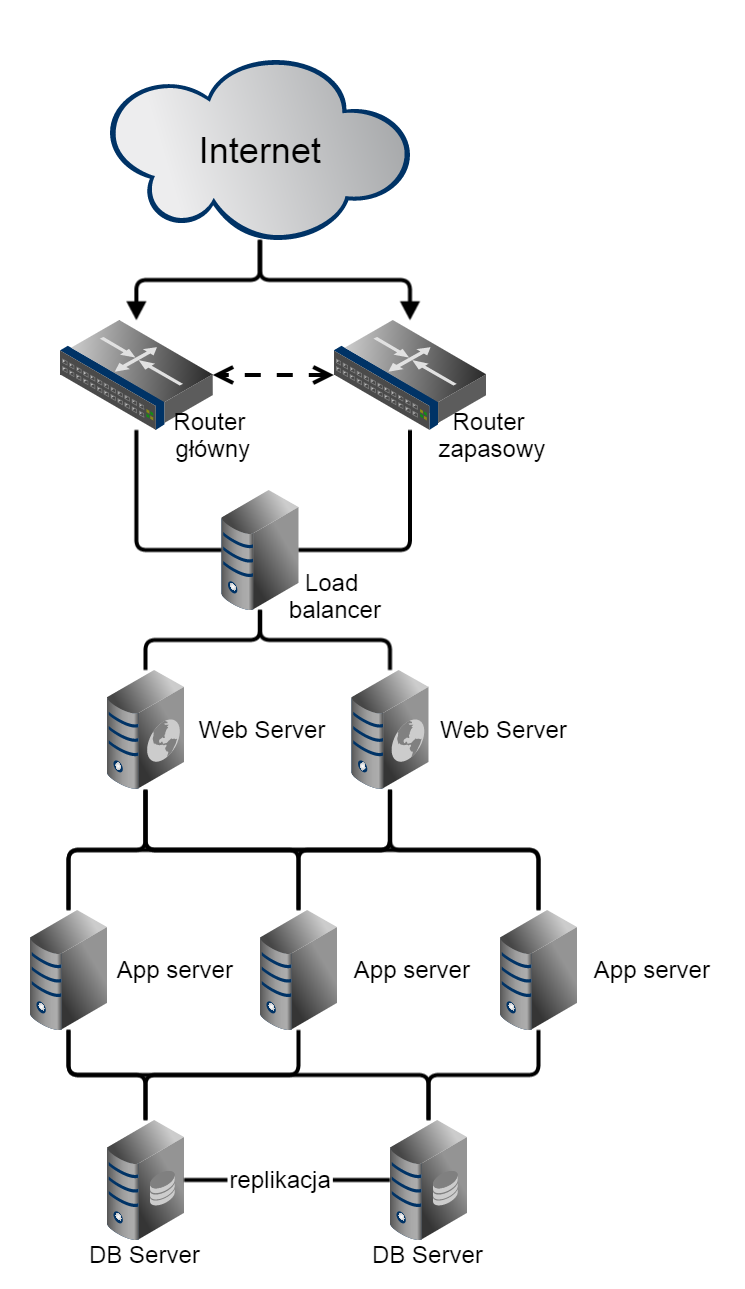
\includegraphics[scale=0.4]{img/architektura}
	\caption{Schemat architektury \label{fig:labelArchitecture}}
\end{figure}

\subsection{Schemat architektury}

Jak uwidoczniono na \ref*{fig:labelArchitecture} na wejściu żądania będą obsługiwany przez router główny, któremu towarzyszył będzie router zapasowy w przypadku, kiedy router główny nie będzie w stanie obsłużyć żądania. Następnie wybierany będzie Web Server, który będzie obsługiwał zgłoszenie (w zależności od poziomu obciążenia serwerów, decydować o tym będzie Load Balancer). W analogiczny sposób wybierany będzie serwer aplikacyjny, pośredniczący w obsłudze.

W odniesieniu do serwerów bazy danych zastosowany będzie mechanizm replikacji danych, który ma zagwarantować bezpieczeństwo przechowywanych informacji (ochronę przed ich utratą w wyniku awarii jednego z serwerów).